%
% File acl2012.tex
%
% Contact: Maggie Li (cswjli@comp.polyu.edu.hk), Michael White (mwhite@ling.osu.edu)
%%
%% Based on the style files for ACL2008 by Joakim Nivre and Noah Smith
%% and that of ACL2010 by Jing-Shin Chang and Philipp Koehn


\documentclass[11pt,letterpaper]{article}

\usepackage[letterpaper]{geometry}
\usepackage{acl2012}
\usepackage{times}
\usepackage{latexsym}
\usepackage{amsmath}
\usepackage{multirow}
\usepackage{url}
\makeatletter
\newcommand{\@BIBLABEL}{\@emptybiblabel}
\newcommand{\@emptybiblabel}[1]{}
\makeatother
\usepackage[hidelinks]{hyperref}
\usepackage{stackrel}
\DeclareMathOperator*{\argmax}{arg\,max}
\setlength\titlebox{4cm}    % Expanding the titlebox

\usepackage{listings}
\usepackage{color}
\usepackage{amsmath}
\usepackage{graphicx}
\graphicspath{ {images/} }

\definecolor{dkgreen}{rgb}{0,0.6,0}
\definecolor{gray}{rgb}{0.5,0.5,0.5}
\definecolor{mauve}{rgb}{0.58,0,0.82}

\lstset{frame=tb,
  language=Java,
  aboveskip=3mm,
  belowskip=3mm,
  showstringspaces=false,
  columns=flexible,
  basicstyle={\small\ttfamily},
  numbers=none,
  numberstyle=\tiny\color{gray},
  keywordstyle=\color{blue},
  commentstyle=\color{dkgreen},
  stringstyle=\color{mauve},
  breaklines=true,
  breakatwhitespace=true,
  tabsize=3
}

\title{Adam Group's Experiements on Chinese-English Machine Translation: Final Project of CMPT413 Winter 2016}

\author{Lyken Zhu \\
  {\tt lykenz@sfu.ca} \\\And
  Jetic Gu \\
  {\tt jeticg@sfu.ca} \\}

\date{}

\begin{document}
\maketitle
\begin{abstract}
  As the final project, we as Adam Group implemented a machine translation system with two different approaches: one with the classical phrase-based decoder and reranker approach, another one with neural network(Neural Machine Translation).  We compared the results of these two different approaches and 
concluded that the Neural Machine Translation is much more superior(BLEU score 0.218) than the traditional phrase-based approach(BLEU score 0.07)
\end{abstract}

\section{Movitation}

The implementation starts with our assignments. Our team’s implementation of decoder and reranker performed quite well, so our first idea is to make them work together, and also try out some new ideas that we didn’t have time for while doing the individual assignments.

We have also attempted to do experiments on a larger scale, by using the large dataset and Gigaword language model, but resulted in failure due to the limitation of our computer. The large dataset combined with Gigaword language model requires too much memory, so we had to abandon the plan. We have also attempted the feedback loop between the decoder and reranker because we wanted to improve the performance.

Last but not least, we also looked at a recent paper \cite{seq2seq} which proposed a state-of-the-art model based on seq2seq LSTMs.

\section{Approach}

\subsection{Phrase-based Approach}
Our first approach is to use our original decoder implementation and reranker implementation. We modified the decoder to generate features and a list of n-best sentences while decoding. We used a textbook translation model:
$$e = \stackrel[e]{}{argmax} Pr(e|f) = argmax\sum_{a} \stackrel[TM]{}{Pr}(f,a|e) * \stackrel[LM]{}{Pr}(e) $$
 
The algorithm we used to perform decoding is simple. Each term, we choose a phrase from the source sentence, and add it to every sentence in the stack. After each term, prune the stack according to their language model scores and translation model scores so that we do not get exponential running time. Here is the pseudocode:

\begin{lstlisting}
# Initialise stack1
add emptySentence to stack1
# start computation
for i=1 to length(f) do
  for phrase in all the phrases from f do
    for sentence in stack1 do
      if phrase not overlap with sentence then
        newSentence = combine(sentence, phrase)
        if translationComplete(newSentence) then
        	add newSentence to answerSet
        else
          add newSentence to stack2
  stack1 = prune(stack2)
  stack2 = emptyStack
# Prune to N-Best
prune(answerSet)
\end{lstlisting}

After retrieving a set of all the answers(answerSet in the algorithm above), we use the features and a weight vector to rerank these sentences, and the sentence with the highest feature score will be the final output.



\subsubsection{The Features}

We used the classic features for our rerankers, including the following:

\begin{itemize}
\itemsep0em 
\item $LMScore$: the language model score for this candidate
\item $ReorderingScore$: the sum of the distortion penalties for this translation
\item $p(f|e)$: the inverse phrase translation probability
\item $lex(f|e)$: the inverse lexical weighting
\item $p(e|f)$: the direct phrase translation probability
\item $lex(e|f)$: the direct lexical weighting
\end{itemize}

All of the features are generated during decoding. For reordering score, we used the following equation to calculate the score:
%EQ2
$$Score=\sum_{d}log(a^{|d|})$$

where d is the distance of the original position of the two adjacent phrases in the target language. We tried several values and settled down for 0.9.

\subsubsection{The Score for Reranking}

The total score for reranking is calculated by the following formula:

$$Score=Feature^T * Weight$$

whereas the weights are calculated by our reranker’s learner. The learner implementation is exactly the same with our assignment implementation, which is basically a pairwise ranking optimisation algorithm given in HW5.

\subsection{Neural Machine Approach}
\label{ssec:first}

Neural Machine Translation (NMT) is a powerful model which achived several state-of-the-art peformances in large-scale translation tasks such as English-French (Luong 2015) and English-Germen (Jean et al. 2015). After studying the results of these papers, we believe it might also show a competitive performance on Chinese to English translation.

The sequence to sequence model is pretty straight-forward:  first the neural machine reads through all of the source words until the $<eos>$ is reached; then RNN units will be used to perform end-to-end trainning.

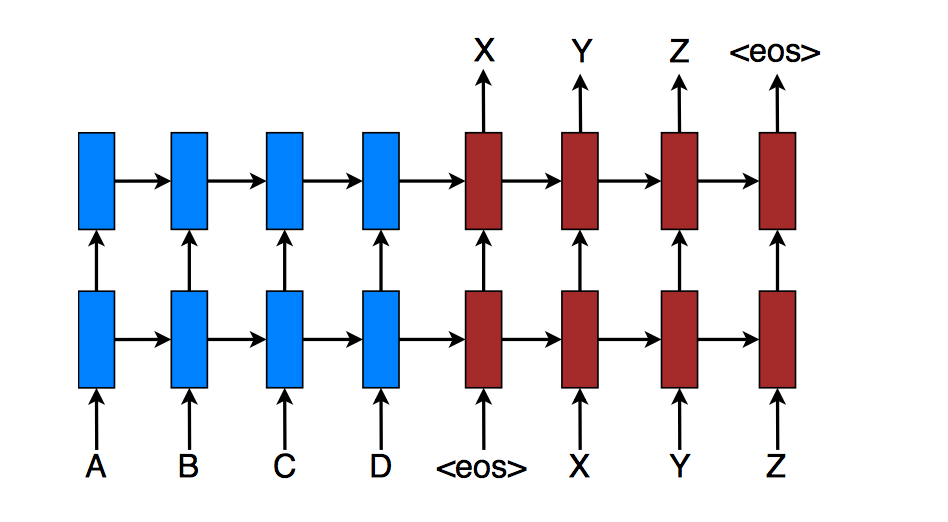
\includegraphics[width=\columnwidth]{seq2seq.png}

As illustraed in the figure above, its size only depends on the length of total words. Because the Gigaword phrase-table is to large for our machines, and the fact that after feeding enough data, a large neural network has the ability to generalise the rules well by itself, we did not use the Gigaword phrase-table.

According to the paper (Mnih et al., 2014), the concept of "attention" improves the score by allowing models to learn alighnments between different modalities. Luong also further explored the use of attention-based architectures of NMT, and achived state-of-the-art in Germen to English translation. Hence, we studied and decided to utilise their design: one global and local attention layer above for a variable length-alignment.



The $\bar{h_s}$ is the source hidden state. 
and $\bar{h_t}$ is the current targe hiddent state.

$$a_t(s)=align(h_t, \bar{h_s})\\
=\frac{exp(score(h_t, \bar{h_s})}{\sum_{s'}exp(score(h_t, \bar{h_{s'}})}$$

Where
\begin{equation}
 score(h_t, \bar{h_{s'}})=
\left\{
\begin{aligned}
h_{t}^{T} * \bar{h_{s'}}  \\
h_{t}^{T} * W_a * \bar{h_{s'}} \\
h_{t}^{T} * tanh(W_a[h_t; \bar{h_{s'}}]) \\ 
\end{aligned}
\right.
\begin{aligned}
dot \\
general\\
concat\\ 
\end{aligned}
\end{equation}

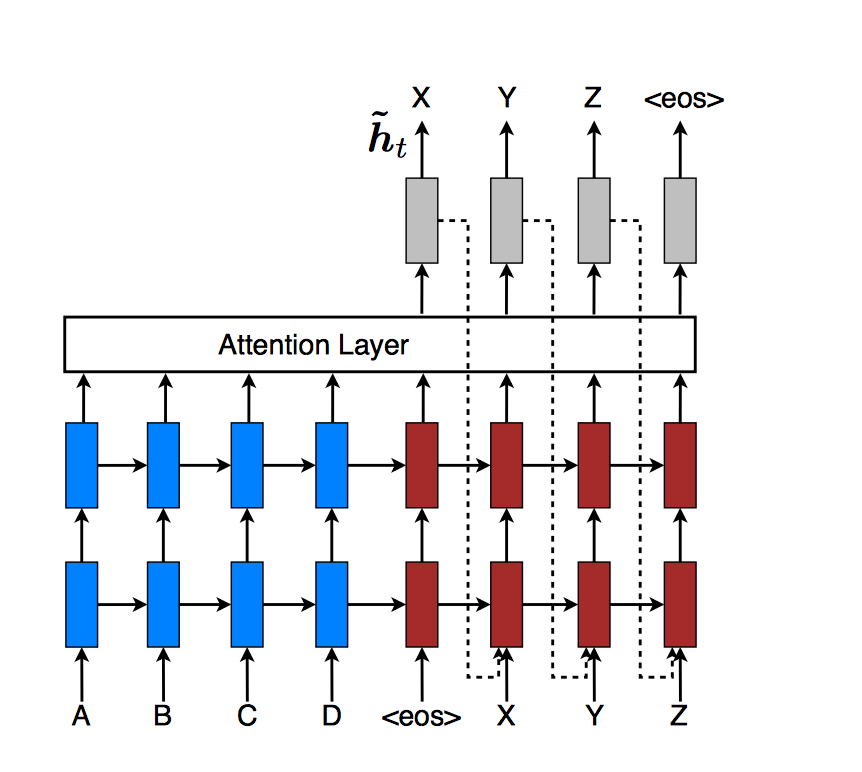
\includegraphics[width=\columnwidth]{attn_layer.png}

\section{Data}

\begin{table}[h]
\begin{center}
\begin{tabular}{|l|r|}
\hline
item & \bf Data  \\ 
\hline
phrase table & filtered-phrase-table\\
language model	&	nlp-data/lm/en.tiny3g.arpa\\
Input		&	nlp-data/medium/train.cn\\
Reference	&	nlp-data/medium/train.en\\
\hline
\end{tabular}
\end{center}
\caption{\label{test-data-pb} test-data for phrase-based model }
\end{table}

\begin{table}[h]
\begin{center}
\begin{tabular}{|l|r|}
\hline
item & \bf Data  \\ 
\hline
alignment	&	nlp-data/meidum/alignemnt\\
Train		&	nlp-data/large (last 40k) \\
Valid		&	nlp-data/medium  \\

\hline
\end{tabular}
\end{center}
\caption{\label{NMT-data-pb} test-data for NMT model }
\end{table}

\section{Code}

Our code consists of two parts: the original implementation, and the NMT.

The code of our phrase-based approach implementation is under the directory `project`, which are all written by ourselves or were provided by the instructor to use during HW1-5.

Our Neural Machine Translation implementation’s main programme is under the directory `seq2seq`. It utilises RNN/GRN frameworks from \cite{RNN} and the skeleton code from Harvard NLP group \cite{seq2seq}


\section{Experimental Setups}
\subsection{Phrase-based approach}

As naive Chinese speakers, we've noticed some imperfection of the segmented data provided for us, such as "Lei Shenglong Yiyuan"(Sheng-long Lei MP) is segmented as "Leisheng Long Yiyuan"(Thunder Long MP). So in addition to using the segmented data, we also used re-segmented data using Stanford segmenter\cite{}, and did the following

1. Generate N-best using the segmented Chinese sentences.

2. Generate weights using the N-best file using our own decoder.

3. Use the our rerank to compute proper weights

4. Use weights to perform translation

\subsection{Neural Machine Approach}
In this approach, we don't need phrase table. All sentences are preprocessed to hdf5 file consumable for Torch.

1. Filter those abitarily long sentence (more than 50 words)

2. Map all appeared EN words and CN phrases into a number

3. Feed into Recurrent Neural Network, and wait patiently.

\section{Results Analysis}
\begin{table}[h]
\begin{center}
\begin{tabular}{|l|r|}
\hline
Method & \bf BLEU  \\ 
\hline
baseline (using filtered table)	&	0.071\\
baseline (using stanford's segmenter)		&	0.076 \\
neural machine approach		&	\textbf{0.218}  \\
\hline
\end{tabular}
\end{center}
\caption{\label{perfm} Performance Comparasion }
\end{table}

Our design of the phrase-based method consists of a lot of parts(segmentation, phrase-table selection, decoding, reranking), and each part is equally influential and therefore important.
During the early tests we have discovered that better segmentation means better quality of translation, but during our implementation of reranker in HW5, we have also noticed irregularities of the reranker on specific datasets, where the error rate might not drop but instead increase as we train the weights. Also, datasets with the same score and close resemblance could also result in dramatically different weights, plus it so happens, we’ve also learned from other groups that the potential benefit of using feedback loop could be very limited. We suspect that this is caused by the amount and type of features we used, and therefore considered the possibility of using neural network to do the translation.

According the the results above, it is within reason to reach the conclusion that Neural Machine Translation does have its superb qualities. Instead of manually selecting and generating features, the End2End model is fully capable of automatically generating its own feature and conduct learning, which justifies its marvellous performance.


\section{Future Work}
As for phrase-based approach, though we would not expect any huge improvement, there are still lots we could do. For example, one could look into the possibility of using a much more efficient decoder implementation, or the option of generating more features for reranking. But as far as BLEU score are concerned, we believe that the neural machine translation might be a better choice. There are still lots of potential options, like embeling segmention into translation, making the whole pipeline end-to-end, adopting residual connections\cite{He2015} which is similar to attention-based to neural network to NLP tasks and inversitaging how depth and length affect the performance of neural network in NLP\cite{NIPS_deep} .

\bibliography{project}
\bibliographystyle{acl2012}

\end{document}



